\documentclass[resume]{subfiles}

\begin{document}
\section{Scheduling}
\begin{itemize}
\item Périodique (time-driven)
\item Apériodique (event-driven)
\item Sporadique (tâches faites au moins tous les $T_{max}$) 
\item Arrière-plan (download)
\end{itemize}

\subsection{Static scheduling}

Fixer lors de l'écriture du code. Impossible de la modifier lors de exécution du code

\subsubsection{Paramètres des tâches}
\begin{itemize}
\item $P_x$ : période de la tâche
\item $D_x$ : deadline
\item $C_x$ : cas le plus long de exécution de la tâche
\item $C_x < P_x$ : cette condition doit toujours être vrai
\item $D_x = P_x$ : simplification 
\end{itemize}

\subsubsection{Marche à suivre (super-loop model)}
\begin{itemize}
\item Définir le plus petit temps d'exécution commun aux tâches

\item Est ce possible de construire une table en prenant compte des deadline (si possible le faire)

\item Exécuter la table des temps sur un cycle

\item Les tâches peuvent être découpées en sous parties (ou ralentie (wait))
\end{itemize}

\subsubsection{Avantages}
\begin{itemize}
\item Facile à implémenter (après avoir trouver la table)
\item Prévisible et facile à debuger
\end{itemize}

\subsubsection{Désavantages}
\begin{itemize}
\item Difficile à trouver la time table (peux être très longue est découpée)
\item Exécution des tâches fixes 
\item Le délais entre deux appelle de tâche est fixe (1cycle complet)
\item Le programme test tout le temps chaque device (polling)
\item Cette méthode s'adapte mal (modification compliqué)
\end{itemize}

\subsection{Event-driven scheduling}

Basé sur des évènements généré par une source et utilisé par le receveur

Les évènements peuvent arriver de manière prévisible (cyclique) ou non (bouton)

Meilleur que la super-loop (pas de polling)(rapidité de gestion des entrée bouton)

\subsubsection{Avantages}
\begin{itemize}
\item Efficace (pas de polling)
\item Rapide (mécanisme hardware) interruption bouton
\item Modifiable (on peut rajouter facilement des ISR)
\end{itemize}

\subsubsection{interruption}

priorité, masquage, imbrication des ISR, allocation de mémoire modifiable 

Opération atomique dans les interruptions, pas d'allocation dynamique, ni d'utilisation de mutex

\subsection{Dynamic scheduling}

Basé sur la priorité des tâches ou durée au choix. L'exécution des tâches va changer durant l'exécution du code

Une tâche ne peux pas être coupée (RTC Run To Completion)

\subsubsection{Marche à suivre}
\begin{itemize}
\item Si pas de tâche prête, il reste en IDLE
\item SI pas de tâche en cours, il démarre la tâche READY la plus prioritaire
\item Lors de l'exécution d'une tâche pas de préemption (RTC)
\item Une fois fini l'exécution la tâche passe en WAITING jusqu'à qu'elle repasse en READY
\end{itemize}

\subsection{Dynamic preemptive scheduling}

Une tâche peut être coupé par une autre tâche plus prioritaire

\subsubsection{Marche à suivre}
\begin{itemize}
\item Une activité de tâche peut être mise en attente (bloquée)
\item Une tâche qui attend ne revient pas au CPU. Elle doit être signalée par une ISR ou une autre tâche
\item Seul le scheduler déplace les tâches entre ready et running
\item Sinon : round-robin entre les tâches de même priorités
\end{itemize}

\subsection{Comparaison des temps de réponse}
\begin{figure}[H]
    \centering
    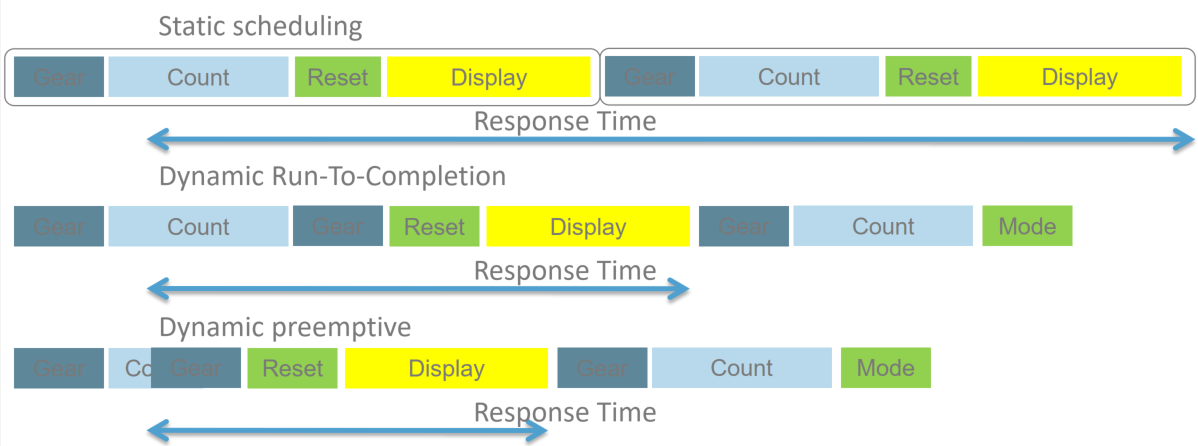
\includegraphics[width=1\columnwidth]{Figures/scheduling/tempsReponse.png}
\end{figure}

\begin{itemize}
\item preemption offre de meilleurs temps de réponse
\item preemption nécessite plus de mémoire et plus complexe
\item preemption introduit des vulnérabilité (mutex déjà utilisé)
\item introduit le concept de RTOS
\end{itemize}

\subsection{Comparaison des performances}
\begin{itemize}


\item Difficile voir impossible de faire des comparaisons définies

\item Il faut à la fois des analyses théoriques et des mesures empiriques
\subitem Analyse théorique : théorie des files, modélisation
\subitem Mesures empiriques : avec de la simulation ou des mesures sur des systèmes existants

\item Mesures de performances
\subitem Temps d'attente : temps perdu par les tâches à attendre lorsqu'elles sont ready
\subitem Temps turnaround : temps pris de la soumission de la tâche à sa complétion
\subitem Utilisation du CPU
\subitem Throughput : nombre de tâches exécutée par unités de temps
\subitem Temps de réponse
\subitem Equitabilité entre tâches

\end{itemize}

















\end{document}